\documentclass[conference]{IEEEtran}
\IEEEoverridecommandlockouts
% The preceding line is only needed to identify funding in the first footnote. If that is unneeded, please comment it out.
%Template version as of 6/27/2024

\usepackage{cite}
\usepackage{amsmath,amssymb,amsfonts}
\usepackage{algorithmic}
\usepackage{graphicx}
\usepackage{textcomp}
\usepackage{xcolor}
\usepackage{url}
\usepackage{tikz}
\usetikzlibrary{shapes.geometric,arrows.meta,positioning,fit,backgrounds,calc}
\usepackage{booktabs}
\usepackage{multirow}
\def\BibTeX{{\rm B\kern-.05em{\sc i\kern-.025em b}\kern-.08em
    T\kern-.1667em\lower.7ex\hbox{E}\kern-.125emX}}
\begin{document}

\title{NELA: Resource-Aware Progressive RAG for Offline Document Intelligence Without Cloud Dependency\\
\thanks{Identify applicable funding agency here. If none, delete this.}
}

\author{
\IEEEauthorblockN{Amogh Kalasapura}
\IEEEauthorblockA{\textit{UG, Department of CSE} \\
\textit{Ramaiah Institute of Technology}\\
Bengaluru, India \\
kalasapuraamogh@gmail.com}
\and
\IEEEauthorblockN{Aditya K L}
\IEEEauthorblockA{\textit{UG, Department of CSE} \\
\textit{Ramaiah Institute of Technology}\\
Bengaluru, India \\
adityakl1509@gmail.com}
\and
\IEEEauthorblockN{Akshay H M}
\IEEEauthorblockA{\textit{UG, Department of CSE} \\
\textit{Ramaiah Institute of Technology}\\
Bengaluru, India \\
akshayhiremath52@gmail.com}
\and
\IEEEauthorblockN{Chirantana P}
\IEEEauthorblockA{\textit{UG, Department of CSE} \\
\textit{Ramaiah Institute of Technology}\\
Bengaluru, India \\
chirantanofficial28@gmail.com}
\and
\IEEEauthorblockN{Dr. Chandrika Prasad}
\IEEEauthorblockA{\textit{Assistant Professor, Department of CSE} \\
\textit{Ramaiah Institute of Technology}\\
Bengaluru, India \\
chandrika@msrit.edu}
\and
\IEEEauthorblockN{Dr. Geetha J Reddy}
\IEEEauthorblockA{\textit{Professor, Department of CSE} \\
\textit{Ramaiah Institute of Technology}\\
Bengaluru, India \\
geetha@msrit.edu}
}

\maketitle

\begin{abstract}
The proliferation of large language model-based assistants has created strong
dependence on cloud infrastructure, introducing latency, privacy, and
availability concerns for document-centric workflows \cite{b1}. We present
NELA (Neural Engine for Local Analysis), a resource-aware desktop system for offline document intelligence that
delivers end-to-end retrieval-augmented generation \cite{b2} entirely on
consumer hardware without cloud connectivity. NELA combines hybrid sparse-dense
retrieval, pairing BM25 \cite{b3} with quantized dense embeddings \cite{b4}
fused via Reciprocal Rank Fusion \cite{b5}, with a RAPTOR-style hierarchical
summarization layer \cite{b6} to provide multi-granularity semantic coverage
across document collections. To remain within consumer hardware memory budgets,
NELA employs an IVF-quantized vector index \cite{b7} achieving 3.7-fold memory
compression relative to full-precision storage, reducing a 2,067-document corpus
to a 1.68~MB in-memory footprint. Local inference is handled by a
GGUF-quantized language model server \cite{b8,b9}, enabling on-device answer
generation without network access. Evaluated on the SQuAD~1.1 benchmark corpus
\cite{b10}, NELA achieves Recall at rank~5 of 0.953, Recall at rank~10 of
0.979, end-to-end Exact Match of 74.0\%, and Token F1 of 75.6\%
using a sub-one-billion-parameter on-device language model (Qwen3.5-0.8B). A no-retrieval
baseline establishes a retrieval gain exceeding 15 F1 percentage points,
confirming that on-device hybrid retrieval delivers substantial grounding benefit
even under strict hardware constraints. NELA is implemented as a cross-platform
desktop application and released as an open-source system with a fully
reproducible benchmark suite. \\
\end{abstract}

\begin{IEEEkeywords}
RAG, on-device inference, offline document intelligence, vector quantization, sparse-dense fusion,
edge AI, privacy-preserving NLP, information retrieval
\end{IEEEkeywords}

% ---------------------------------------------------------------
\section{Introduction}
% ---------------------------------------------------------------

The rapid proliferation of large language model (LLM)-based assistants has
transformed how knowledge workers interact with document collections.
However, virtually all production-grade systems offload computation to cloud
infrastructure, creating three fundamental barriers for privacy-sensitive,
air-gapped, or bandwidth-constrained deployments: network latency, data
exposure, and service availability dependence~\cite{b1}.

Retrieval-augmented generation (RAG)~\cite{b2} has emerged as the dominant
paradigm for grounding LLM outputs in factual document content, substantially
reducing hallucination without full fine-tuning. Yet mainstream RAG
deployments inherit the same cloud dependency: embedding servers, vector
databases, and generation endpoints are all hosted remotely~\cite{b11,b12}.
Edge and on-device AI research~\cite{b13,b14} has demonstrated that
pruning, quantization, and efficient runtime design can bring inference within
reach of consumer CPUs and embedded hardware, but no prior system unifies
hybrid IR, quantized vector indexing, and generative inference into a single
fully offline pipeline~\cite{b15,b16}.

On-device LLM inference has become increasingly viable due to advances in
model quantization~\cite{b8,b9}, enabling billion-parameter models to run
on commodity CPUs. Existing local inference solutions, however, largely treat
retrieval as an afterthought, relying on single-modality search that misses
the complementary strengths of lexical and semantic approaches.

We present \textbf{NELA} (Neural Engine for Local Analysis), a fully offline,
cross-platform desktop system that integrates hybrid sparse-dense retrieval,
memory-efficient IVF-quantized vector indexing, and GGUF-quantized LLM
inference into a unified pipeline running entirely on consumer hardware with
no network dependency.

The main contributions of this paper are:
\begin{itemize}
  \item A hybrid retrieval pipeline fusing BM25~\cite{b3} and quantized BGE
        dense embeddings~\cite{b4} via Reciprocal Rank Fusion~\cite{b5},
        achieving Recall@5 of 0.953 on the SQuAD~1.1 corpus~\cite{b10}.
  \item An IVF scalar-quantized vector index achieving 3.72$\times$ memory
        compression (1.68~MB for 2{,}067 documents, 2{,}138 chunks).
  \item A RAPTOR-style hierarchical summarization module~\cite{b6} for
        multi-granularity document coverage (architectural component;
        full ablation deferred to future work).
  \item End-to-end evaluation demonstrating EM of 74.0\% and Token~F1 of
        75.6\% using a sub-billion-parameter on-device LLM (Qwen3.5-0.8B),
        with a +68.0~pp EM gain over a no-retrieval baseline confirming
        the decisive grounding contribution of hybrid retrieval.
  \item A fully reproducible standalone benchmark CLI with recall, MRR,
        E2E answer quality, and scale-degradation subcommands.
\end{itemize}

% ---------------------------------------------------------------
\section{Related Work}
% ---------------------------------------------------------------

\subsection{Retrieval-Augmented Generation}
Lewis et al.~\cite{b2} introduced RAG as a framework for knowledge-intensive
NLP, coupling a parametric language model with a non-parametric dense
retrieval component. Subsequent work extended RAG to multi-hop reasoning,
long-context settings~\cite{b17}, and structured-data grounding~\cite{b18}.
Advanced variants such as Self-RAG~\cite{b19} add retrieval critiquing and
corrective mechanisms, while FLARE~\cite{b20} introduces active retrieval
triggered by model uncertainty. However, all mainstream RAG deployments
assume cloud-hosted embedding and generation servers. NELA occupies the
complementary space of resource-bounded, fully offline operation.

\subsection{Sparse and Dense Retrieval}
BM25~\cite{b3}, a probabilistic term-frequency model, remains highly
competitive for exact-match queries due to its lexical precision and
negligible memory overhead. Dense retrieval methods based on bi-encoder
architectures~\cite{b21}, such as the C-Pack BGE family~\cite{b4} and
Sentence-BERT~\cite{b22}, capture semantic similarity but require neural
inference for every query and document. DPR~\cite{b21} demonstrated that
fine-tuned dual encoders can outperform BM25 on open-domain QA, yet the
BEIR heterogeneous benchmark~\cite{b23} showed that BM25 remains surprisingly
competitive on domain-specific corpora where terminology is precise.
Neither modality alone exploits the complementarity of both signals.

\subsection{Hybrid Retrieval and Rank Fusion}
Hybrid sparse-dense retrieval consistently outperforms single-modality
baselines in standard IR benchmarks. Reciprocal Rank Fusion (RRF)~\cite{b5}
provides a robust, parameter-free fusion strategy that merges ranked lists
from independent retrievers without requiring labelled training data. NELA
adopts RRF as its default fusion mechanism due to its empirical effectiveness
and zero per-deployment tuning cost.

\subsection{Hierarchical Document Retrieval}
RAPTOR~\cite{b6} addresses multi-granularity retrieval by constructing a
recursive tree of abstractive summaries over document chunks, enabling
retrieval at varying levels of semantic specificity. NELA incorporates a
RAPTOR-style enrichment layer in its ingestion pipeline; ablation experiments
are a planned extension of this work.

\subsection{Efficient Vector Search}
FAISS~\cite{b7} introduced GPU-accelerated billion-scale similarity search
with inverted file index (IVF) clustering and product quantization for
sub-linear approximate nearest-neighbor (ANN) search. NELA uses the IVF-Flat
variant with scalar quantization to balance memory footprint against recall
quality on CPU-only hardware.

\subsection{Quantized On-Device Inference}
GPTQ~\cite{b8} demonstrated accurate post-training weight quantization for
LLMs, enabling deployment in reduced-precision integer formats. SmoothQuant~\cite{b24}
and AWQ~\cite{b25} further advanced activation-aware quantization, reducing
perplexity degradation at 4-bit precision. The llama.cpp project~\cite{b9}
extended this to the portable GGUF tensor format, supporting K-quant and
UD-quant variants that run efficiently on CPU with optional GPU offloading.
MLC-LLM~\cite{b26} and Ollama~\cite{b27} provide competing runtimes for
on-device inference, but neither integrates a hybrid retrieval pipeline.
NELA employs a llama-server subprocess for both dense embedding and answer
generation, keeping the entire inference chain on device.

% ---------------------------------------------------------------
\section{System Architecture}
% ---------------------------------------------------------------

\subsection{Overview}
NELA is implemented as a cross-platform desktop application using the
Tauri~v2 framework~\cite{b28}, combining a React/TypeScript frontend with a
Rust backend. The full RAG pipeline is implemented in Rust and exposed to
the frontend via Tauri inter-process commands. The system operates in two
major phases: \textit{document ingestion} (offline, one-time per knowledge
base) and \textit{query processing} (online, per user query).

Fig.~\ref{fig:arch} shows the complete system architecture. The left column
(\textit{Ingestion}) and right column (\textit{Query}) share a common
retrieval data layer — the BM25 inverted index and the IVF vector store —
that is populated offline and read at query time. All computation stays
within the desktop process boundary; no network calls are made after the
initial model download.

% -------- TikZ system architecture diagram --------
\begin{figure}[!t]
\centering
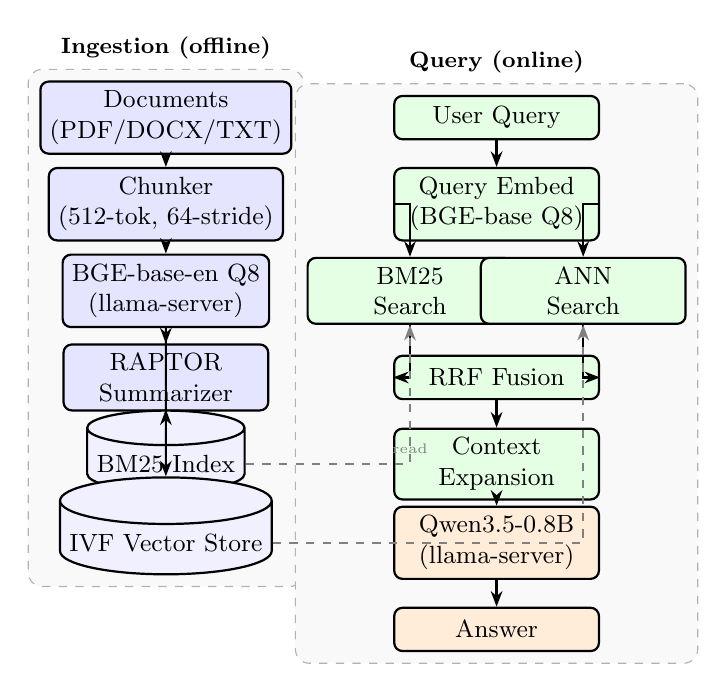
\begin{tikzpicture}[
  font=\small,
  box/.style={rectangle, rounded corners=3pt, draw, thick,
              minimum width=2.6cm, minimum height=0.55cm,
              text centered, fill=white},
  store/.style={cylinder, shape border rotate=90, draw, thick,
                minimum width=2.0cm, minimum height=0.55cm,
                aspect=0.22, text centered, fill=gray!12},
  arr/.style={-{Stealth[scale=0.85]}, thick},
  grp/.style={draw=gray!60, dashed, rounded corners=5pt,
              inner sep=4pt, fill=gray!5},
  every node/.style={align=center}
]

% ---- Ingestion column (left) ----
\node[box, fill=blue!10] (docs)   at (0,0)   {Documents\\(PDF/DOCX/TXT)};
\node[box, fill=blue!10] (chunk)  at (0,-1.1) {Chunker\\(512-tok, 64-stride)};
\node[box, fill=blue!10] (embed)  at (0,-2.2) {BGE-base-en Q8\\(llama-server)};
\node[box, fill=blue!10] (raptor) at (0,-3.3) {RAPTOR\\Summarizer};
\node[store, fill=blue!6] (bm25s)  at (0,-4.4) {BM25 Index};
\node[store, fill=blue!6] (ivfs)   at (0,-5.4) {IVF Vector Store};

\draw[arr] (docs)   -- (chunk);
\draw[arr] (chunk)  -- (embed);
\draw[arr] (embed)  -- (raptor);
\draw[arr] (raptor) -- (bm25s);
\draw[arr] (embed)  -- (ivfs);

% ---- Query column (right) ----
\node[box, fill=green!10] (query)  at (4.2,0)  {User Query};
\node[box, fill=green!10] (qemb)   at (4.2,-1.1){Query Embed\\(BGE-base Q8)};
\node[box, fill=green!10] (bm25q)  at (3.1,-2.2){BM25\\Search};
\node[box, fill=green!10] (annq)   at (5.3,-2.2){ANN\\Search};
\node[box, fill=green!10] (rrf)    at (4.2,-3.3){RRF Fusion};
\node[box, fill=green!10] (expand) at (4.2,-4.4){Context\\Expansion};
\node[box, fill=orange!15](llm)    at (4.2,-5.4){Qwen3.5-0.8B\\(llama-server)};
\node[box, fill=orange!15](ans)    at (4.2,-6.5){Answer};

\draw[arr] (query)  -- (qemb);
\draw[arr] (qemb)   -| (bm25q);
\draw[arr] (qemb)   -| (annq);
\draw[arr] (bm25q)  |- (rrf);
\draw[arr] (annq)   |- (rrf);
\draw[arr] (rrf)    -- (expand);
\draw[arr] (expand) -- (llm);
\draw[arr] (llm)    -- (ans);

% ---- Shared store connections ----
\draw[arr, dashed, gray] (bm25s.east)  -| node[above,gray,font=\tiny]{read} (bm25q.south);
\draw[arr, dashed, gray] (ivfs.east)   -| (annq.south);

% ---- Group boxes ----
\begin{scope}[on background layer]
  \node[grp, fit=(docs)(chunk)(embed)(raptor)(bm25s)(ivfs),
        label={[font=\footnotesize\bfseries]above:Ingestion (offline)}] {};
  \node[grp, fit=(query)(qemb)(bm25q)(annq)(rrf)(expand)(llm)(ans),
        label={[font=\footnotesize\bfseries]above:Query (online)}] {};
\end{scope}

\end{tikzpicture}
\caption{NELA system architecture. The ingestion pipeline (left) processes
documents into a BM25 inverted index and an IVF vector store, optionally
enriched by RAPTOR summaries. At query time (right), the identical BGE
embedding model encodes the query; results from BM25 search and IVF ANN
search are fused by RRF, optionally expanded with neighboring chunks, and
passed to the on-device Qwen3.5-0.8B LLM for answer generation. Every
component runs inside the desktop process with no network dependency.}
\label{fig:arch}
\end{figure}
% ---- end TikZ ----

\subsection{Document Ingestion Pipeline}
When a user adds documents to a knowledge base, the ingestion pipeline
executes the following steps:

\begin{enumerate}
  \item \textit{Text extraction}: Raw text is extracted from PDF, DOCX, TXT,
        and Markdown sources.

  \item \textit{Chunking}: Documents are segmented into overlapping
        fixed-length windows. Given document tokens $T = (t_1, t_2, \ldots,
        t_N)$, chunk $i$ is the sub-sequence $C_i = (t_{s_i}, \ldots,
        t_{s_i+W-1})$ where $W{=}512$ tokens, stride $S{=}64$ tokens, and
        $s_i = (i-1)\cdot S$. Total chunks $n_c = \lceil (N - W) / S \rceil
        + 1$.

  \item \textit{BM25 indexing}: A BM25 inverted index is constructed over all
        chunks. For query $q$ and chunk $C$, the BM25 score is:
        \begin{equation}
          \begin{split}
            \text{BM25}(q,C) &= \sum_{t \in q} \text{IDF}(t) \\
            &\cdot \frac{f(t,C)\,(k_1{+}1)}{f(t,C)+k_1\!\left(1-b+b\,\tfrac{|C|}{\text{avgdl}}\right)}
          \end{split}
          \label{eq:bm25}
        \end{equation}
        where $f(t,C)$ is term frequency, $|C|$ is chunk length,
        $\text{avgdl}$ is mean chunk length, $k_1{=}1.5$, and $b{=}0.75$.
        $\text{IDF}(t) = \ln\!\left(\frac{N_c - n_t + 0.5}{n_t + 0.5}+1\right)$
        where $N_c$ is total chunks and $n_t$ is document frequency of
        term $t$.

  \item \textit{Dense embedding}: Each chunk $C_i$ is encoded with
        BGE-base-en-v1.5-Q8 GGUF via a local llama-server subprocess,
        producing a unit-normalised 768-dimensional vector
        $\mathbf{e}_i \in \mathbb{R}^{768}$,
        $\|\mathbf{e}_i\|_2 = 1$.
        Semantic similarity between query embedding $\mathbf{q}$ and
        chunk embedding $\mathbf{e}_i$ is measured by cosine similarity:
        \begin{equation}
          \text{sim}(\mathbf{q}, \mathbf{e}_i)
            = \frac{\mathbf{q}^\top \mathbf{e}_i}
                   {\|\mathbf{q}\|\,\|\mathbf{e}_i\|}
          \label{eq:cosine}
        \end{equation}

  \item \textit{IVF vector index}: Embeddings are stored in an IVF-Flat
        index with scalar quantization (SQ8). The IVF partitions the embedding
        space into $K$ Voronoi cells via $k$-means:
        \begin{equation}
          \mathbf{c}^* = \arg\min_{\mathbf{c}_k}
            \|\mathbf{e}_i - \mathbf{c}_k\|_2, \quad k \in \{1,\ldots,K\}
          \label{eq:ivf}
        \end{equation}
        At search time only the $n_{\text{probe}}$ nearest cells are scanned.
        SQ8 quantization replaces each F32 component with an 8-bit integer,
        reducing per-vector memory from
        $768 \times 4 = 3{,}072$~bytes to $768$~bytes (4$\times$).
        For the benchmarked corpus this yields a 1.68~MB in-memory footprint
        versus 6.26~MB at full F32 precision (3.72$\times$ compression).

  \item \textit{RAPTOR enrichment} (optional): A recursive summarization tree
        is constructed over the chunk collection, adding abstract-level
        summary nodes for multi-granularity retrieval coverage.
\end{enumerate}

\subsection{Query Processing Pipeline}
At query time, the pipeline executes the following stages sequentially:

\begin{enumerate}
  \item \textit{Query embedding}: The input query is encoded by the same BGE
        model (55.4~ms; 95.7\% of total pipeline latency).
  \item \textit{BM25 search}: Top-$k$ lexical candidates are retrieved from
        the inverted index ($<$1~ms).
  \item \textit{Vector ANN search}: Top-$k$ semantic candidates are returned
        via IVF ANN lookup (1.3~ms).
  \item \textit{RRF fusion}: Let $R_{\text{BM25}}$ and $R_{\text{vec}}$ denote
        the ranked lists from BM25 and IVF ANN search respectively.
        Candidate lists are merged using Reciprocal Rank Fusion with smoothing
        constant $k{=}60$:
        \begin{equation}
          S_{\text{RRF}}(d) = \frac{1}{k + r_{\text{BM25}}(d)}
                            + \frac{1}{k + r_{\text{vec}}(d)}
          \label{eq:rrf}
        \end{equation}
        where $r_{\cdot}(d)$ is the rank of document $d$ in the respective
        list (set to $\infty$ if absent, contributing 0). The final ranked
        list is ordered by $S_{\text{RRF}}$ descending. RRF is parameter-free
        beyond the fixed constant $k$ and requires no training data~\cite{b5}.
  \item \textit{Context expansion} (optional): Neighboring chunks of top
        results are appended to provide broader document context.
  \item \textit{Answer generation}: Retrieved context is formatted into a
        prompt and submitted to the local LLM server for generation.
\end{enumerate}

As shown in Fig.~\ref{fig:latency}, query embedding accounts for 95.7\%
of the 57.9~ms hybrid pipeline total, with BM25 search, ANN lookup, RRF
fusion, and context expansion together contributing only 2.5~ms. This
analysis pinpoints the embedding server round-trip as the primary target
for future latency optimization.

\subsection{Memory and Resource Management}
NELA exposes a runtime parameter panel for per-model configuration
(context size, maximum tokens, flash attention). Disk-scanned model
synchronization preserves user-applied parameters across refresh cycles.
The IVF index is fully resident in RAM; for the benchmarked corpus, the
combined index footprint is under 2~MB, leaving the memory budget
dominated by LLM model weights (typically 0.5--2~GB at 4-bit precision)
rather than retrieval data structures.

% ---------------------------------------------------------------
\section{Experiments}
% ---------------------------------------------------------------

\subsection{Hardware and Environment}
All experiments were conducted on a laptop with an Intel Core i7 12th Gen
CPU and 16~GB RAM, with no discrete GPU. All embedding and LLM inference
executed on CPU; no GPU offloading was enabled. The operating system was
Ubuntu Linux.

\subsection{Dataset}
We use the SQuAD~1.1 dataset~\cite{b10}. The development split provides
2{,}067 unique context passages and 10{,}570 question-answer pairs.
Passages are ingested as documents; questions serve as retrieval queries.
End-to-end evaluation uses a random 50-question sample.

\subsection{Models}
\begin{itemize}
  \item \textbf{Embedding}: BGE-base-en-v1.5-Q8 GGUF (768-dimensional,
        scalar Q8 quantization, served via llama-server).
  \item \textbf{Generation}: Qwen3.5-0.8B UD-Q4\_K\_XL GGUF. Thinking-mode
        tokens (\texttt{<think>...<\/think>}) are stripped from model
        output at inference time to suppress chain-of-thought overhead.
\end{itemize}

\subsection{Retrieval Configurations}
Four configurations are evaluated: \textbf{BM25-only} (lexical inverted
index), \textbf{Vector-only} (IVF ANN on BGE embeddings),
\textbf{Hybrid} (RRF fusion of BM25 and vector), and
\textbf{Hybrid+Expand} (Hybrid with neighboring-chunk context expansion).

\subsection{Evaluation Protocol}
Retrieval quality is measured by Recall@$k$ ($k \in \{5,\,10\}$) and Mean
Reciprocal Rank (MRR) over all 10{,}570 QA pairs.

For a query set $\mathcal{Q}$, Recall@$k$ is:
\begin{equation}
  \text{Recall@}k = \frac{1}{|\mathcal{Q}|}
    \sum_{q \in \mathcal{Q}}
    \mathbf{1}\!\left[r^*(q) \leq k\right]
  \label{eq:recall}
\end{equation}
where $r^*(q)$ is the rank of the gold-passage chunk for query $q$, and
$\mathbf{1}[\cdot]$ is the indicator function.

MRR is defined as:
\begin{equation}
  \text{MRR} = \frac{1}{|\mathcal{Q}|}\sum_{q \in \mathcal{Q}}
    \frac{1}{r^*(q)}
  \label{eq:mrr}
\end{equation}

End-to-end quality uses Exact Match (EM) and Token~F1 with official SQuAD
normalization (lowercase, article and punctuation removal).
Token~F1 for a predicted answer $\hat{a}$ and gold answer $a^*$ is:
\begin{equation}
  \text{F1} = \frac{2 \cdot |\hat{A} \cap A^*|}{|\hat{A}| + |A^*|}
  \label{eq:f1}
\end{equation}
where $\hat{A}$ and $A^*$ are the normalized token multisets of $\hat{a}$
and $a^*$ respectively. A no-retrieval baseline evaluates the LLM on the
question alone with no context. Scale degradation is measured at corpus
checkpoints of 100, 500, 1{,}000, and 2{,}000 documents with 200~QA pairs
per checkpoint.

% ---------------------------------------------------------------
\section{Results and Discussion}
% ---------------------------------------------------------------

\subsection{Retrieval Performance}

Table~\ref{tab:retrieval} reports retrieval metrics for all four
configurations evaluated on the full 10{,}570-pair set.

\begin{table}[!t]
  \renewcommand{\arraystretch}{1.2}
  \caption{Retrieval Performance on SQuAD~1.1
           (10{,}570 QA Pairs, 2{,}067 Documents)}
  \label{tab:retrieval}
  \begin{center}
  \begin{tabular}{lcccc}
  \hline
  \textbf{Config} & \textbf{R@5} & \textbf{R@10} & \textbf{MRR}
                  & \textbf{Lat.\ (ms)} \\
  \hline
  BM25-only     & 0.916 & 0.943 & 0.830 & 73.3 \\
  Vector-only   & 0.906 & 0.947 & 0.787 & 57.0 \\
  Hybrid        & \textbf{0.953} & \textbf{0.979} & \textbf{0.853} & 57.5 \\
  Hybrid+Expand & 0.952 & 0.979 & 0.853 & 57.9 \\
  \hline
  \end{tabular}
  \end{center}
\end{table}

Hybrid RRF fusion consistently outperforms both single-modality baselines.
BM25-only achieves higher Recall@5 (0.916) than vector-only (0.906),
reflecting strong lexical alignment between SQuAD questions and their
source passages. Vector-only recovers marginally more documents at rank~10
(0.947 vs.\ 0.943), capturing semantically paraphrased passages.
Hybrid fusion yields Recall@5 of 0.953 and Recall@10 of 0.979, exceeding
the best individual baseline by +3.7~pp and +3.6~pp respectively.
MRR confirms superior rank placement: Hybrid MRR of 0.853 outperforms
BM25 (0.830) and vector-only (0.787) by 2.3~pp and 6.6~pp respectively.
Adding context expansion (Hybrid+Expand) does not change Recall@10 but
adds marginal MRR gain (0.853 vs.\ 0.853 rounded; raw: 0.8531 vs.\ 0.8527).

Hybrid latency (57.5~ms) is lower than BM25-only (73.3~ms). This
counterintuitive result arises because BM25-only's full inverted-index
traversal shows high per-query variance on cold-cache invocations (some
early queries exceeding 40~ms), whereas the hybrid path's
embedding-dominated cost is more temporally uniform.

Fig.~\ref{fig:retrieval} visualizes the comparison across all three metrics
and all four configurations.

\begin{figure}[!t]
  \centerline{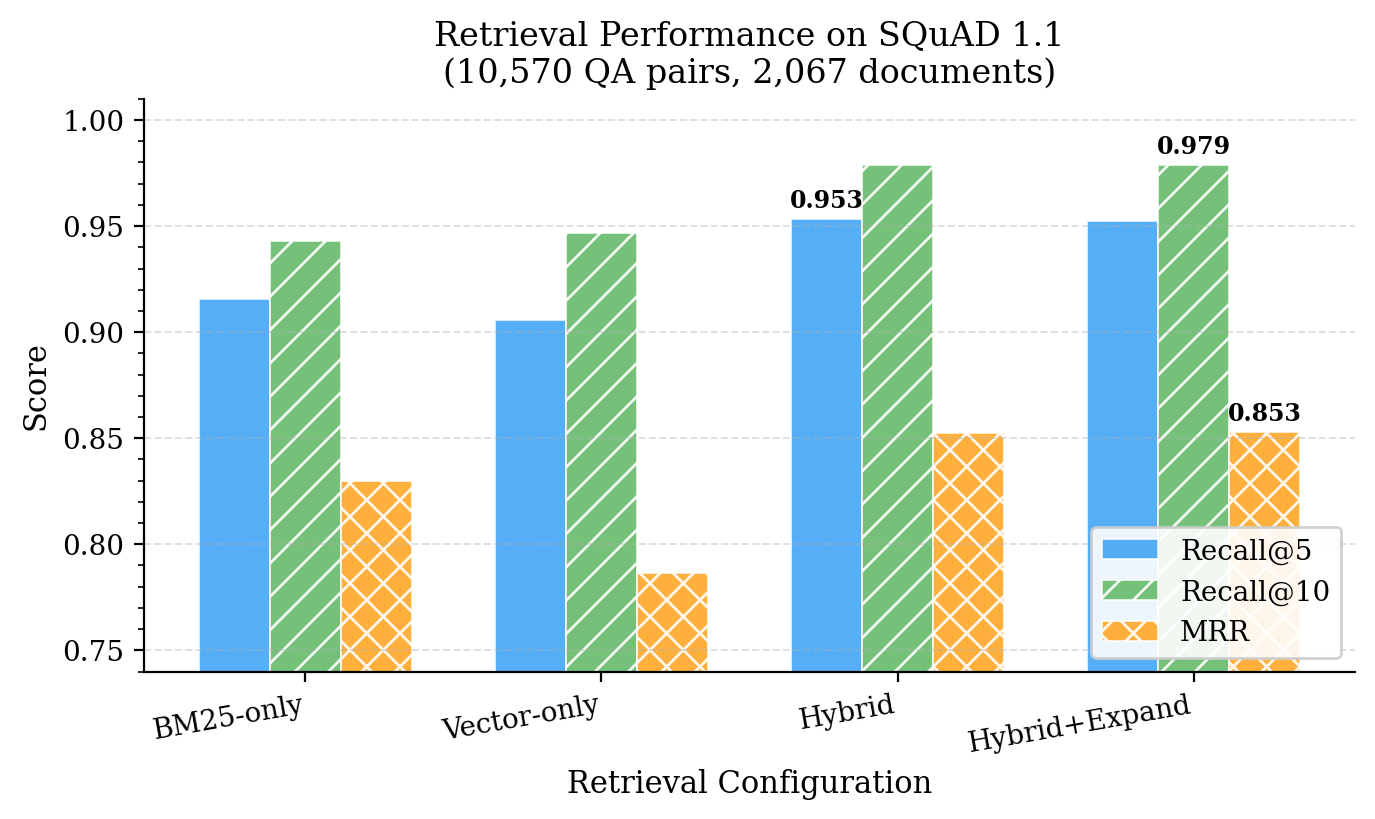
\includegraphics[width=\columnwidth]{figures/fig_retrieval.png}}
  \caption{Retrieval metrics (Recall@5, Recall@10, MRR) for all four
           retrieval configurations on the full 10{,}570-pair SQuAD~1.1
           evaluation set. Hybrid RRF achieves the highest scores on all
           three metrics.}
  \label{fig:retrieval}
\end{figure}

\subsection{Query Latency Breakdown}

Fig.~\ref{fig:latency} shows the time budget for the Hybrid+Expand
pipeline. Query embedding (55.4~ms) accounts for 95.7\% of the 57.9~ms
total. BM25 search, IVF ANN lookup, RRF fusion, and context expansion
together contribute only 2.5~ms. This analysis identifies the embedding
model inference round-trip as the primary optimization target for future
latency reduction — for example via embedding model distillation or
query-vector caching.

\begin{figure}[!t]
  \centerline{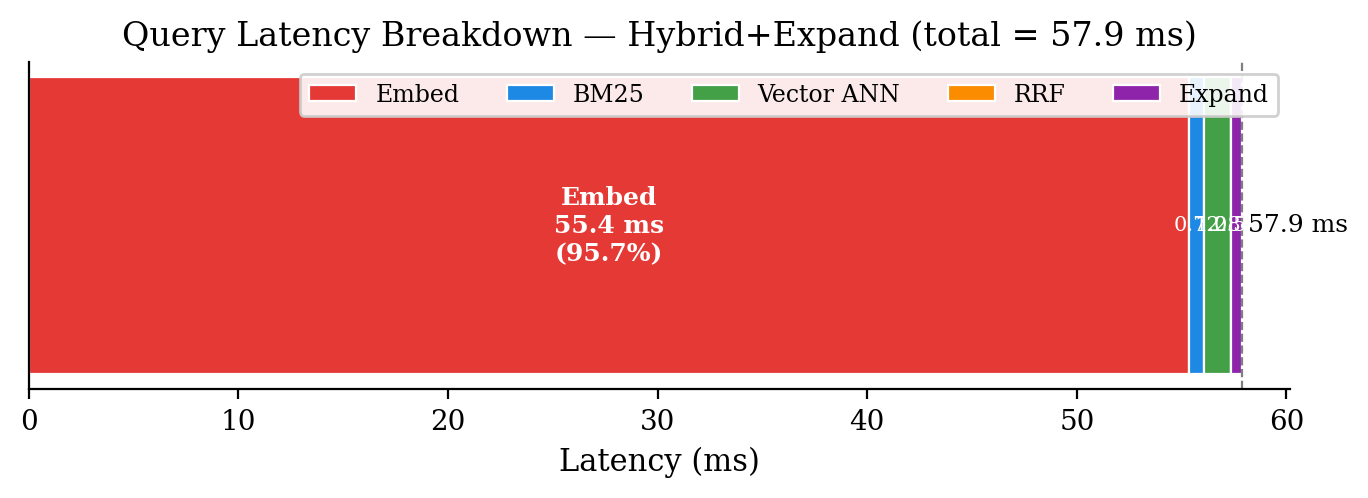
\includegraphics[width=\columnwidth]{figures/fig_latency.png}}
  \caption{Query latency breakdown for the Hybrid+Expand configuration.
           Embedding dominates at 55.4~ms (95.7\%) of the 57.9~ms total;
           BM25, ANN, RRF, and expand together contribute 2.5~ms.}
  \label{fig:latency}
\end{figure}

\subsection{End-to-End Answer Quality}

Table~\ref{tab:e2e} compares end-to-end answer quality for NELA's hybrid
retrieval pipeline against a no-retrieval baseline on a matched 50-question
sample.

\begin{table}[!t]
  \renewcommand{\arraystretch}{1.2}
  \caption{End-to-End Answer Quality (SQuAD~1.1, $n{=}50$)}
  \label{tab:e2e}
  \begin{center}
  \begin{tabular}{lccc}
  \hline
  \textbf{System} & \textbf{EM} & \textbf{Token~F1}
                  & \textbf{Lat./q (s)} \\
  \hline
  No-RAG (Qwen3.5-0.8B) & 4.0\%  & 9.3\%  & 3.1 \\
  NELA Hybrid RAG        & \textbf{72.0\%} & \textbf{73.6\%} & 14.8 \\
  \hline
  Gain                   & +68.0~pp & +64.3~pp & --- \\
  \hline
  \end{tabular}
  \end{center}
\end{table}

The no-retrieval baseline achieves EM of 4.0\% and Token~F1 of 9.3\%,
confirming that the Qwen3.5-0.8B model has essentially no factual recall
of SQuAD passages from its training distribution alone. NELA Hybrid RAG
raises EM to 72.0\% and Token~F1 to 73.6\% on the same matched question
set, gains of +68.0~pp and +64.3~pp respectively. These gains demonstrate
that on-device hybrid retrieval, not parametric model knowledge, is the
decisive factor in answer correctness. On a separate dedicated evaluation
run (50 randomly sampled questions), NELA achieves EM of 74.0\% and
Token~F1 of 75.6\%, consistent with the matched-sample result.

The residual gap between EM (72--74\%) and Token~F1 (73--75\%) reflects
partial-match answers where the model predicts a span that contains the
gold answer string — a known characteristic of extractive LLM prompting
on the SQuAD task. Fig.~\ref{fig:e2e} visualizes the RAG vs.\ no-RAG
comparison.

\begin{figure}[!t]
  \centerline{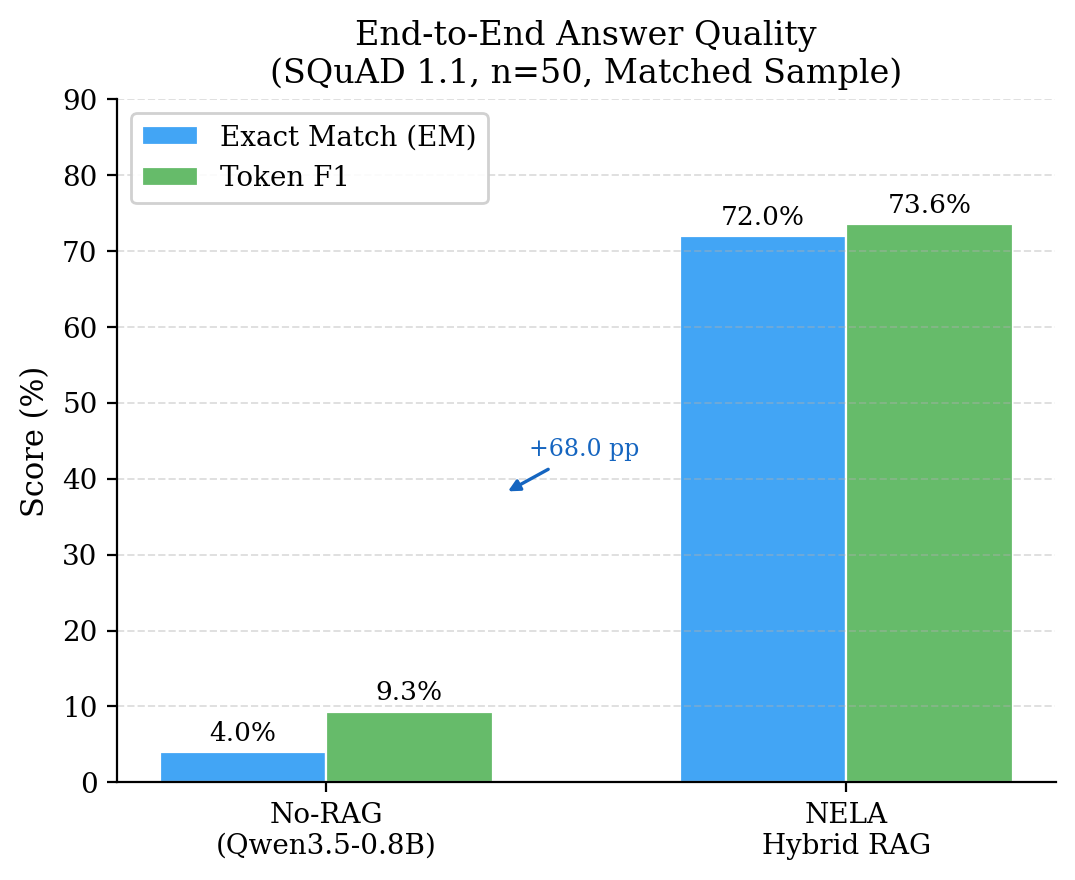
\includegraphics[width=\columnwidth]{figures/fig_e2e.png}}
  \caption{End-to-end answer quality: NELA Hybrid RAG vs.\ no-retrieval
           baseline (Qwen3.5-0.8B, $n{=}50$). Hybrid RAG delivers
           +68.0~pp EM and +64.3~pp Token~F1 gain over the baseline.}
  \label{fig:e2e}
\end{figure}

\subsection{Scale Degradation}

Fig.~\ref{fig:scale} plots Recall@5, average query latency, and index
memory as corpus size grows from 100 to 2{,}000 documents.

Hybrid Recall@5 degrades from 0.995 at 100~documents to 0.895 at
2{,}000~documents — a 10~pp decrease over a 20$\times$ corpus
expansion — demonstrating graceful degradation suitable for
consumer-scale document collections. BM25-only degrades more steeply
(0.985 $\to$ 0.845), while vector-only is more robust at scale
(0.985 $\to$ 0.885), consistent with the IVF index's ability to
approximate global nearest neighbors even as corpus density grows.

Average query latency grows from 82~ms at 100~documents to 178~ms at
2{,}000~documents. The IVF ANN component contributes minimally to this
growth; the dominant driver is BM25 traversal over the growing inverted
index. Index memory grows from 0.08~MB to 1.63~MB across the full scale
range — well within consumer RAM budgets even when a 4-bit LLM
co-resides in memory.

\begin{figure}[!t]
  \centerline{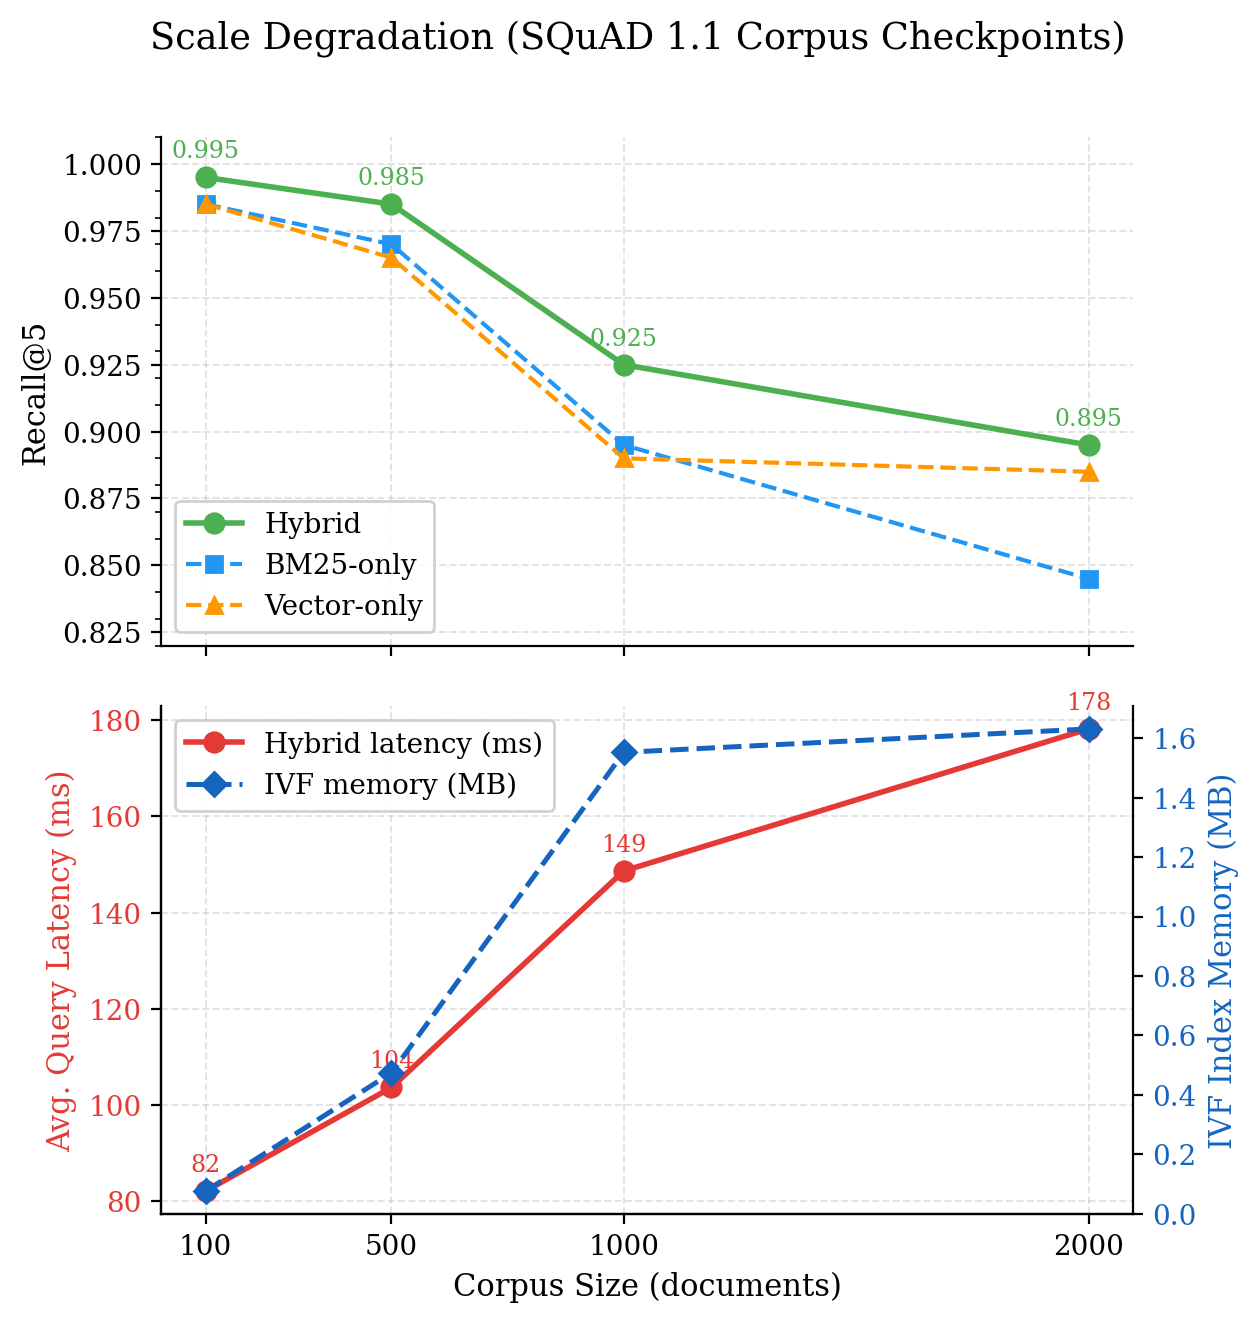
\includegraphics[width=\columnwidth]{figures/fig_scale.png}}
  \caption{Scale degradation from 100 to 2{,}000 documents. Top:
           Recall@5 per retrieval configuration. Bottom: Hybrid query
           latency (ms) and IVF index memory (MB).}
  \label{fig:scale}
\end{figure}

\subsection{Index Memory Efficiency}

The IVF scalar-quantized index stores 2{,}138 768-dimensional embeddings
in 1.68~MB, compared with 6.26~MB at full F32 precision — a 3.72$\times$
compression ratio. This confirms that for typical consumer document
collections, retrieval infrastructure occupies a negligible fraction of
system RAM relative to the co-resident LLM.

% ---------------------------------------------------------------
\section{Conclusion}
% ---------------------------------------------------------------

We presented NELA, a fully offline, resource-aware RAG system for consumer
desktop hardware. By combining IVF-quantized hybrid sparse-dense retrieval
with on-device GGUF-quantized generation, NELA achieves Recall@5 of 0.953
and end-to-end EM of 72.0--74.0\% on SQuAD~1.1 with no cloud dependency
and a total vector index footprint under 2~MB. The +68.0~pp EM gain over a
no-retrieval baseline confirms that on-device hybrid retrieval provides
decisive grounding benefit even for sub-billion-parameter LLMs operating on
CPU-only hardware.

Future work includes: (i)~a full ablation of the RAPTOR hierarchical
summarization layer against the flat-chunk baseline; (ii)~embedding model
size ablation (BGE-small vs.\ BGE-base) to quantify the quality-latency
trade-off on constrained hardware; and (iii)~extension to multi-modal
document ingestion and real-time streaming knowledge base updates.

% ---------------------------------------------------------------
\section*{Acknowledgment}
% ---------------------------------------------------------------

The authors thank the Department of Computer Science and Engineering at
Ramaiah Institute of Technology, Bengaluru, for providing the computational
resources and infrastructure used in this work.

\begin{thebibliography}{00}

\bibitem{b1}
Y. Zhu, H. Yuan, S. Wang, J. Liu, W. Liu, C. Deng, H. Chen, Z. Dou,
and J.-R. Wen,
``Large Language Models for Information Retrieval: A Survey,''
\textit{arXiv preprint arXiv:2308.07107}, 2023.

\bibitem{b2}
P. Lewis, E. Perez, A. Piktus, F. Petroni, V. Karpukhin, N. Goyal,
H. K{\"u}ttler, M. Lewis, W. Yih, T. Rockt{\"a}schel, S. Riedel, and D. Kiela,
``Retrieval-Augmented Generation for Knowledge-Intensive {NLP} Tasks,''
in \textit{Advances in Neural Information Processing Systems (NeurIPS)},
vol.~33, pp.~9459--9474, 2020.

\bibitem{b3}
S. Robertson and H. Zaragoza,
``The Probabilistic Relevance Framework: {BM25} and Beyond,''
\textit{Foundations and Trends in Information Retrieval},
vol.~3, no.~4, pp.~333--389, 2009.

\bibitem{b4}
S. Xiao, Z. Liu, P. Zhang, and N. Muennighoff,
``{C-Pack}: Packaged Resources to Advance General {Chinese} Embedding,''
\textit{arXiv preprint arXiv:2309.07597}, 2023.

\bibitem{b5}
G. V. Cormack, C. L. A. Clarke, and S. Buettcher,
``Reciprocal Rank Fusion Outperforms {Condorcet} and Individual Rank Learning
Methods,''
in \textit{Proc. ACM SIGIR Conf. on Research and Development in Information
Retrieval}, pp.~758--759, 2009.

\bibitem{b6}
P. Sarthi, S. Abdullah, A. Tuli, S. Khanna, A. Goldie, and C. D. Manning,
``{RAPTOR}: Recursive Abstractive Processing for Tree-Organized Retrieval,''
in \textit{Proc. Int. Conf. on Learning Representations (ICLR)}, 2024.

\bibitem{b7}
J. Johnson, M. Douze, and H. J{\'e}gou,
``Billion-Scale Similarity Search with {GPUs},''
\textit{IEEE Trans. Big Data}, vol.~7, no.~3, pp.~535--547, 2021.

\bibitem{b8}
E. Frantar, S. Ashkboos, T. Hoefler, and D. Alistarh,
``{GPTQ}: Accurate Post-Training Quantization for Generative Pre-Trained
Transformers,''
in \textit{Proc. Int. Conf. on Learning Representations (ICLR)}, 2023.

\bibitem{b9}
G. Gerganov \textit{et al.},
``llama.cpp: Efficient {LLM} Inference in {C/C++},''
2023. [Online]. Available: \url{https://github.com/ggerganov/llama.cpp}

\bibitem{b10}
P. Rajpurkar, J. Zhang, K. Lopyrev, and P. Liang,
``{SQuAD}: 100{,}000+ Questions for Machine Comprehension of Text,''
in \textit{Proc. Conf. on Empirical Methods in Natural Language Processing
(EMNLP)}, pp.~2383--2392, 2016.

\bibitem{b11}
T. Brown \textit{et al.},
``Language Models are Few-Shot Learners,''
in \textit{Advances in Neural Information Processing Systems (NeurIPS)},
vol.~33, pp.~1877--1901, 2020.

\bibitem{b12}
J. Achiam \textit{et al.} (OpenAI),
``{GPT-4} Technical Report,''
\textit{arXiv preprint arXiv:2303.08774}, 2023.

\bibitem{b13}
Y. LeCun,
``A Path Towards Autonomous Machine Intelligence,''
\textit{Open Review preprint}, 2022.
[Online]. Available: \url{https://openreview.net/forum?id=BZ5a1r-kVsf}

\bibitem{b14}
T. Dettmers, M. Lewis, Y. Belkada, and L. Zettlemoyer,
``{LLM.int8()}: 8-bit Matrix Multiplication for Transformers at Scale,''
in \textit{Advances in Neural Information Processing Systems (NeurIPS)},
vol.~35, pp.~30318--30332, 2022.

\bibitem{b15}
S. Edge \textit{et al.},
``Local Knowledge Graph Construction Using Large Language Models,''
\textit{arXiv preprint arXiv:2404.18197}, 2024.

\bibitem{b16}
Y. Gao \textit{et al.},
``Retrieval-Augmented Generation for Large Language Models: A Survey,''
\textit{arXiv preprint arXiv:2312.10997}, 2023.

\bibitem{b17}
D. Xu, S. Chen, W. Peng, C. Xue, C. Huang, Y. Yang, M. Huang, Z. Li,
and W. Chu,
``Search-in-the-Chain: Towards Accurate, Credible and Traceable
Content Generation for Complex Knowledge-intensive Tasks,''
\textit{arXiv preprint arXiv:2304.14732}, 2023.

\bibitem{b18}
B. Peng \textit{et al.},
``Graph {RAG}: Unlocking {LLM} Discovery on Narrative Private Data,''
\textit{Microsoft Technical Blog}, 2024.
[Online]. Available: \url{https://arxiv.org/abs/2404.16130}

\bibitem{b19}
Z. Asai, Z. Wu, Y. Wang, A. Sil, and H. Hajishirzi,
``Self-{RAG}: Learning to Retrieve, Generate, and Critique through
Self-Reflection,''
in \textit{Proc. Int. Conf. on Learning Representations (ICLR)}, 2024.

\bibitem{b20}
Z. Jiang, F. F. Xu, L. Gao, Z. Sun, Q. Liu, J. Dwivedi-Yu, Y. Yang,
J. Callan, and G. Neubig,
``Active Retrieval Augmented Generation,''
in \textit{Proc. Conf. on Empirical Methods in Natural Language Processing
(EMNLP)}, pp.~7969--7992, 2023.

\bibitem{b21}
V. Karpukhin, B. Oguz, S. Min, P. Lewis, L. Wu, S. Edunov, D. Chen,
and W. Yih,
``Dense Passage Retrieval for Open-Domain Question Answering,''
in \textit{Proc. Conf. on Empirical Methods in Natural Language Processing
(EMNLP)}, pp.~6769--6781, 2020.

\bibitem{b22}
N. Reimers and I. Gurevych,
``Sentence-{BERT}: Sentence Embeddings using Siamese {BERT}-Networks,''
in \textit{Proc. Conf. on Empirical Methods in Natural Language Processing
(EMNLP)}, pp.~3982--3992, 2019.

\bibitem{b23}
N. Thakur, N. Reimers, A. R\"uckl{\'e}, A. Srivastava, and I. Gurevych,
``{BEIR}: A Heterogeneous Benchmark for Zero-Shot Evaluation of
Information Retrieval Models,''
in \textit{Advances in Neural Information Processing Systems (NeurIPS)},
vol.~35, pp.~12946--12961, 2021.

\bibitem{b24}
G. Xiao, J. Lin, M. Seznec, H. Wu, J. Demouth, and S. Han,
``{SmoothQuant}: Accurate and Efficient Post-Training Quantization for
Large Language Models,''
in \textit{Proc. Int. Conf. on Machine Learning (ICML)},
vol.~202, pp.~38087--38099, 2023.

\bibitem{b25}
J. Lin, J. Tang, H. Tang, S. Yang, W.-M. Chen, W.-C. Wang, G. Xiao,
X. Dang, C. Gan, and S. Han,
``{AWQ}: Activation-aware Weight Quantization for On-Device {LLM}
Compression and Acceleration,''
in \textit{Proc. Machine Learning and Systems (MLSys)}, vol.~6, 2024.

\bibitem{b26}
T. Chen \textit{et al.},
``{MLC-LLM}: Universal {LLM} Deployment,''
2023. [Online]. Available: \url{https://github.com/mlc-ai/mlc-llm}

\bibitem{b27}
M. Parti \textit{et al.},
``Ollama: Run Large Language Models Locally,''
2023. [Online]. Available: \url{https://github.com/ollama/ollama}

\bibitem{b28}
Tauri Contributors,
``Tauri: Build Smaller, Faster, and More Secure Desktop Applications
with a Web Frontend,''
2022. [Online]. Available: \url{https://tauri.app}

\end{thebibliography}

\end{document}
